\documentclass{standalone}
\usepackage{pgfplots}
\usepgfplotslibrary{fillbetween}
\pgfplotsset{compat=1.13}

\begin{document}

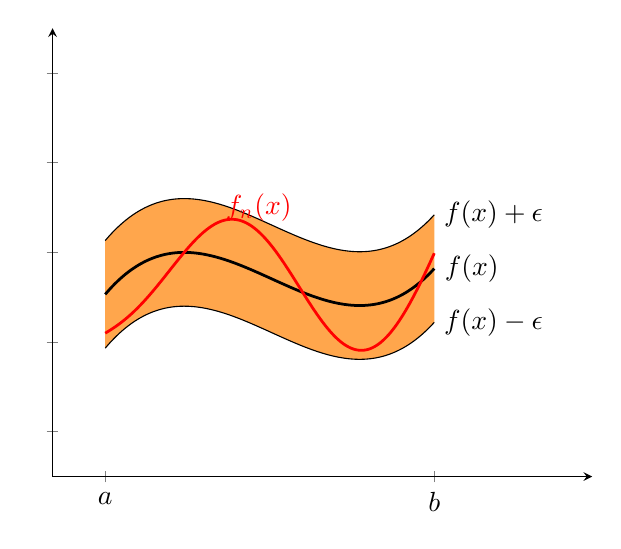
\begin{tikzpicture}
    \begin{axis}[
            axis y line = left,
            axis x line = bottom,
            xtick       = {-1.2,3.8},
            xticklabels = {$a$,$b$},
            yticklabels=\empty,
            samples     = 160,
            domain      = -1.2:3.8,
            xmin = -2, xmax = 6.2,
            ymin = -5, ymax = 5,
            % small,
            % xlabel={\(x\)},
            % ylabel={\(y\)}
        ]
        \addplot[name path=top, black, mark=none, ] {x^3/8-x^2/2 + 1.2} node[right]{\(f(x) + \epsilon\)};
        \addplot[black, mark=none, line width=1pt] {x^3/8-x^2/2 } node[right]{\(f(x)\)};
        \addplot[red, mark=none, line width=1pt] {x^3/8-x^2/2 + sin(100*x)} node[pos=0.4, anchor = south]{\(f_n(x)\)};
        \addplot[name path=bottom, black, no markers] {x^3/8-x^2/2 - 1.2} node[right]{\(f(x) - \epsilon\)};
        \addplot fill between[
                of = top and bottom,
                every even segment/.style = {orange!70},
            ];
    \end{axis}
\end{tikzpicture}

\end{document}